% A1.2 — Final comparison report. Compile with XeLaTeX (see latexmkrc).
\documentclass[11pt, a4paper]{article}
\usepackage{bkreport}

\renewcommand{\reporttitleshort}{A1.2 -- CNN vs Transformer}
\hypersetup{
  pdftitle  = {A1.2\_CNN\_vs\_Transformer\_Report\_Hummingbird},
  pdfauthor = {Nguyen Le Hoang Hung, Nguyen Thi Linh Trang}}
\graphicspath{{../../results/}}

\begin{document}

\makecover{Bài tập lớn A1: CNN vs Transformer trên tập ảnh lớn}
          {Mốc A1.2 -- Báo cáo so sánh cuối}
          {TP. Hồ Chí Minh, ngày 09 tháng 11 năm 2026}

\begin{abstract}
Bài so sánh ResNet-50 (CNN) và DeiT-Small (Transformer), hai mô hình cùng quy mô khoảng 22--24 triệu tham số, trên một subset có kiểm soát của Food-101 (101 lớp; 10.100 ảnh train, 5.050 ảnh test), mỗi mô hình ở bốn chế độ: from-scratch, freeze backbone, freeze một nửa và full finetune. Kết quả tốt nhất là DeiT-S full finetune với 76,20\% top-1, so với 60,44\% của ResNet-50. Pretrain ImageNet là yếu tố quyết định: from-scratch chỉ đạt 17,8\% (ResNet-50) và 11,0\% (DeiT-S). Với DeiT-S, freeze một nửa backbone giữ được 75,39\% top-1 (kém full finetune 0,8 điểm) với một nửa số tham số được train, thời gian train ít hơn 34\% và bộ nhớ GPU bằng khoảng một nửa. Do giới hạn thời gian GPU, quy mô dữ liệu và số epoch nhỏ hơn protocol A1.1; các thay đổi được nêu rõ ở Mục 4.3.
\end{abstract}

\tableofcontents
\newpage

% =====================================================================
\section{Giới thiệu}

CNN mang sẵn \emph{inductive bias} về tính cục bộ và bất biến tịnh tiến, còn Vision Transformer~\cite{dosovitskiy2021vit} xử lý ảnh như một dãy patch và học quan hệ giữa chúng bằng self-attention, gần như không có giả định nào về cấu trúc ảnh. Hệ quả thường được nhắc tới là ViT cần nhiều dữ liệu hoặc cần pretrain mới đạt được độ chính xác của CNN. Bài này kiểm tra nhận định đó trên Food-101~\cite{bossard2014food}, với một CNN (ResNet-50~\cite{he2016resnet}) và một Transformer cùng quy mô (DeiT-Small~\cite{touvron2021deit}), mỗi mô hình ở bốn chế độ huấn luyện.

Các câu hỏi nghiên cứu (giữ nguyên từ A1.1):
\begin{enumerate}
  \item Khi train from-scratch, CNN hay ViT tốt hơn? Vì sao?
  \item Pretrain giúp mỗi họ kiến trúc bao nhiêu? ViT có cần pretrain nhiều hơn CNN không?
  \item Khi nào freeze có lợi và khi nào nên full finetune?
  \item Đánh đổi giữa accuracy và chi phí của từng cấu hình là gì?
\end{enumerate}

% =====================================================================
\section{Dataset và EDA}

\subsection{Food-101}
Food-101~\cite{bossard2014food} gồm 101 lớp món ăn, 750 ảnh train và 250 ảnh test mỗi lớp, ảnh màu có cạnh dài tối đa 512 px. Ảnh lấy từ foodspotting.com, chỉ dùng cho nghiên cứu và học tập; repo không chứa ảnh, chỉ chứa code tải dữ liệu. Split train gốc có nhiễu nhãn do tác giả cố ý giữ lại, còn split test đã được làm sạch thủ công. Food-101 không phải tập con của ImageNet, nên các mô hình pretrained ImageNet không bị rò dữ liệu test.

\subsection{Split}

Tất cả split được lấy phân tầng theo lớp với seed 42 bằng \code{scripts/prepare\_data.py}; danh sách ảnh nằm trong \code{A1/splits/} (Bảng~\ref{tab:split}). Validation dùng để chọn checkpoint (epoch có top-1 validation cao nhất); test chỉ dùng một lần cho mỗi run.

\begin{table}[H]
  \centering
  \caption{Cách chia dữ liệu (seed 42, phân tầng theo lớp).}
  \label{tab:split}
  \begin{tabular}{llrr}
    \toprule
    \textbf{Split} & \textbf{Nguồn} & \textbf{Ảnh/lớp} & \textbf{Tổng} \\
    \midrule
    Train      & split train gốc & 100 & 10.100 \\
    Validation & split train gốc, không giao với Train & 20 & 2.020 \\
    Test       & split test gốc (đã làm sạch) & 50 & 5.050 \\
    \bottomrule
  \end{tabular}
\end{table}

\subsection{Phân tích dữ liệu}

Ba split cân bằng tuyệt đối theo cách lấy mẫu (cùng số ảnh mỗi lớp), nên accuracy và macro-F1 có ý nghĩa tương đương và không cần trọng số lớp. Ảnh gốc có cạnh dài đúng 512 px (trung vị 512 px, đo trên 2020 ảnh train lấy mẫu); 62\% là ảnh vuông, phần còn lại có tỉ lệ khung hình khác nhau (Hình~\ref{fig:eda-sizes}). Vì vậy resize về cạnh ngắn 256 px rồi center crop 224 px giữ được gần trọn món ăn ở phần lớn ảnh.

\begin{figure}[H]
  \centering
  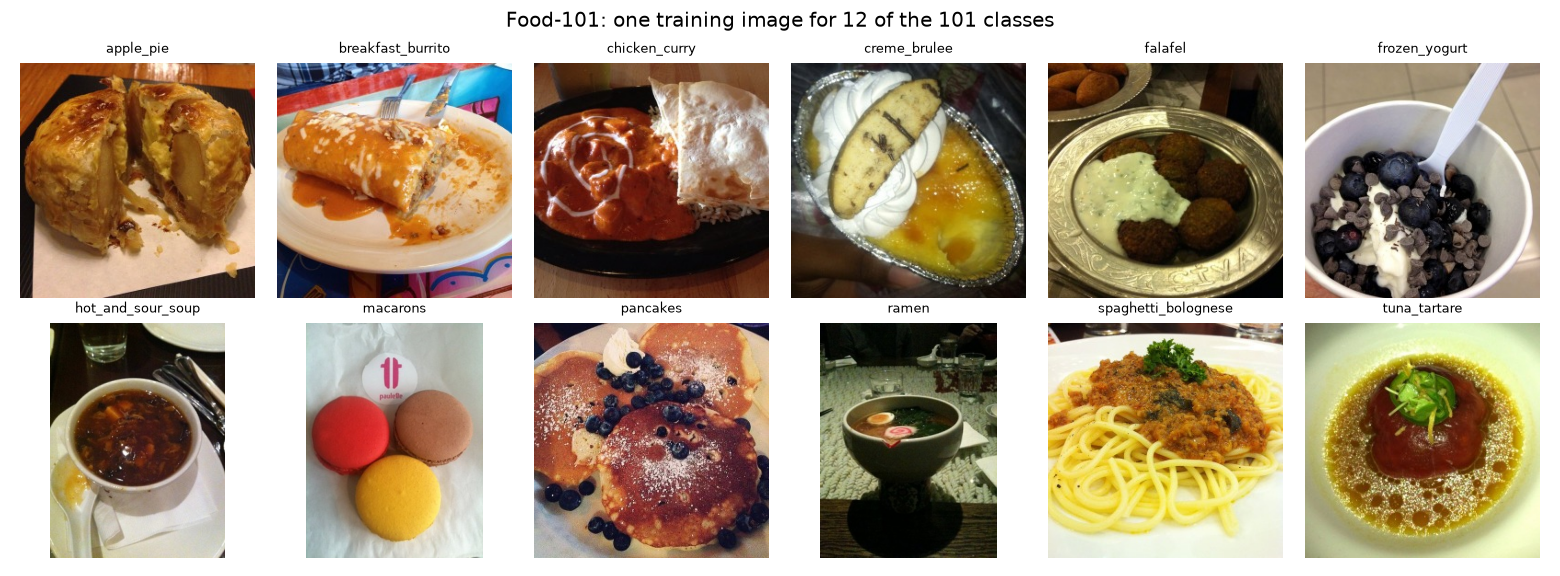
\includegraphics[width=\linewidth]{fig_eda_samples.png}
  \caption{Một ảnh train của 12 trong 101 lớp. Ảnh chụp tự nhiên, góc chụp, ánh sáng và bố cục rất khác nhau.}
  \label{fig:eda-samples}
\end{figure}

\begin{figure}[H]
  \centering
  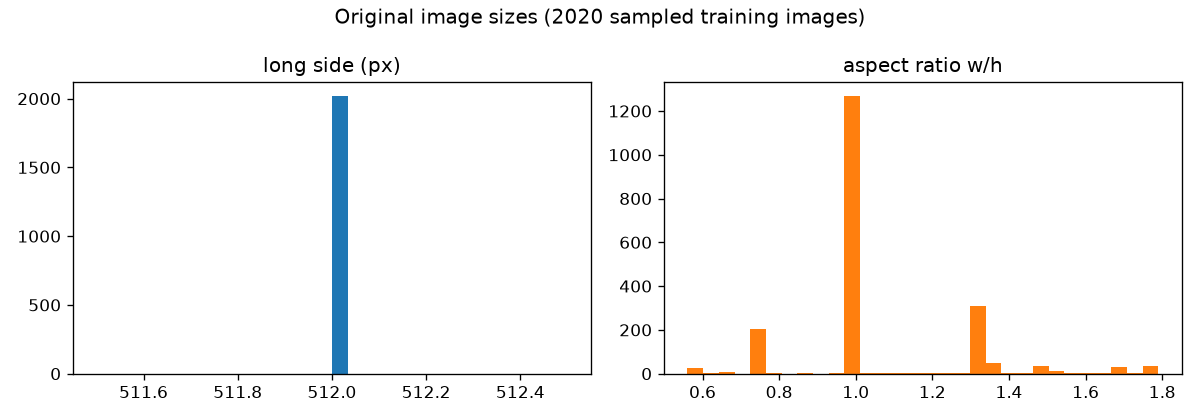
\includegraphics[width=0.85\linewidth]{fig_eda_sizes.png}
  \caption{Kích thước ảnh gốc: cạnh dài và tỉ lệ khung hình.}
  \label{fig:eda-sizes}
\end{figure}

% =====================================================================
\section{DataLoader và Augmentation}

Ảnh được resize một lần về cạnh ngắn 256 px (\code{prepare\_data.py}, dùng \code{Image.draft} để giải mã JPEG ở độ phân giải thấp), vì giải mã ảnh gốc 512 px trên CPU là nút thắt của DataLoader. Chuẩn hóa theo mean/std của ImageNet.

\textbf{Train:}
\begin{lstlisting}
RandomResizedCrop(224, scale=(0.35, 1.0))
RandomHorizontalFlip(p=0.5)
TrivialAugmentWide()
ToTensor(), Normalize(mean, std)
RandomErasing(p=0.25)
\end{lstlisting}

\textbf{Validation / Test:}
\begin{lstlisting}
Resize(256), CenterCrop(224)
ToTensor(), Normalize(mean, std)
\end{lstlisting}

DataLoader: batch 64, 8 worker, \code{pin\_memory}, thứ tự xáo trộn cố định bằng generator có seed. Mọi run dùng cùng pipeline, nên giữa hai run chỉ khác kiến trúc hoặc chế độ huấn luyện. TrivialAugment~\cite{muller2021trivialaugment} không cần tinh chỉnh tham số; Random Erasing~\cite{zhong2020randomerasing} giảm overfit.

% =====================================================================
\section{Protocol thí nghiệm}

\subsection{Mô hình và chế độ huấn luyện}

\begin{table}[H]
  \centering
  \caption{Hai mô hình (checkpoint \code{timm}~\cite{wightman2019timm}, pretrained ImageNet-1k). Head luôn được khởi tạo lại cho 101 lớp.}
  \label{tab:models}
  \begin{tabular}{llrr}
    \toprule
    \textbf{Mô hình} & \textbf{Checkpoint} & \textbf{Tổng tham số} & \textbf{Head} \\
    \midrule
    ResNet-50~\cite{he2016resnet}     & \code{resnet50.a1\_in1k}~\cite{wightman2021rsb} & 23.714.981 & 206.949 \\
    DeiT-Small~\cite{touvron2021deit} & \code{deit\_small\_patch16\_224.fb\_in1k}        & 21.704.549 & 38.885 \\
    \bottomrule
  \end{tabular}
\end{table}

\begin{table}[H]
  \centering
  \caption{Bốn chế độ huấn luyện và số tham số được train.}
  \label{tab:modes}
  \small
  \begin{tabularx}{\linewidth}{lYrr}
    \toprule
    \textbf{Chế độ} & \textbf{Phần được train} & \textbf{ResNet-50} & \textbf{DeiT-S} \\
    \midrule
    From-scratch    & Toàn bộ, khởi tạo ngẫu nhiên & 23,71M & 21,70M \\
    Freeze backbone & Chỉ head (linear probe) & 0,21M & 0,04M \\
    Freeze một nửa  & ResNet: \code{layer3}, \code{layer4}, \code{fc}; DeiT: \code{blocks[6:12]}, \code{norm}, \code{head} & 22,27M & 10,69M \\
    Full finetune   & Toàn bộ, khởi tạo ImageNet & 23,71M & 21,70M \\
    \bottomrule
  \end{tabularx}
\end{table}

Với ResNet, các lớp BatchNorm thuộc phần bị freeze được đặt ở chế độ \code{eval()} sau mỗi lần \code{model.train()}, để giữ nguyên running statistics của ImageNet (24 lớp BN ở chế độ freeze một nửa, cả 53 lớp ở chế độ freeze backbone). Phần freeze một nửa của ResNet chiếm 7/16 bottleneck block nhưng chỉ khoảng 6\% tham số, vì các tầng đầu ít kênh; phần freeze của DeiT chiếm đúng một nửa tham số vì 12 block có cùng kích thước.

\subsection{Huấn luyện}

Training loop tự viết (\code{src/train.py}): forward $\rightarrow$ cross-entropy với label smoothing 0,1~\cite{szegedy2016rethinking} $\rightarrow$ \code{backward()} $\rightarrow$ \code{optimizer.step()}. AdamW~\cite{loshchilov2019adamw}, warm-up tuyến tính 10\% số bước đầu rồi cosine~\cite{loshchilov2017sgdr} về 0, mixed precision fp16~\cite{micikevicius2018mixed}. Bias và tham số LayerNorm/BatchNorm không chịu weight decay.

\begin{table}[H]
  \centering
  \caption{Hyperparameter (learning rate và weight decay theo protocol A1.1).}
  \label{tab:hparams}
  \begin{tabular}{lcccc}
    \toprule
    \textbf{Chế độ} & \textbf{Epoch} & \textbf{LR head} & \textbf{LR backbone} & \textbf{Weight decay} \\
    \midrule
    From-scratch    & 10 & $10^{-3}$ & $10^{-3}$ & 0,05 \\
    Freeze backbone & 5  & $10^{-3}$ & --        & $10^{-4}$ \\
    Freeze một nửa  & 5  & $10^{-3}$ & $10^{-4}$ & 0,05 \\
    Full finetune   & 5  & $10^{-3}$ & $10^{-4}$ & 0,05 \\
    \bottomrule
  \end{tabular}
\end{table}

\paragraph{Phần cứng.} NVIDIA GeForce GTX 1070 (8GB, Pascal), PyTorch 2.8 bản CUDA 12.6. Đo trên máy này: AMP fp16 nhanh hơn fp32 khoảng 29\% với ResNet-50 (142 so với 110 ảnh/s) và 19\% với DeiT-S (114 so với 96 ảnh/s), đồng thời giảm gần một nửa bộ nhớ, nên mọi run dùng AMP.

\subsection{Thay đổi so với protocol A1.1}

Protocol A1.1 cần ước tính 12--15 giờ GPU; tại thời điểm chạy chỉ còn khoảng 2 giờ trước hạn nộp. Thiết kế thí nghiệm (2 mô hình $\times$ 4 chế độ, cùng split, augmentation, learning rate, weight decay cho mọi run) được giữ nguyên; chỉ quy mô bị giảm (Bảng~\ref{tab:deviations}). Mọi kết luận bên dưới cần đọc trong bối cảnh này: số liệu tuyệt đối thấp hơn mức có thể đạt được, đặc biệt ở hai run from-scratch.

\begin{table}[H]
  \centering
  \caption{Những điểm khác protocol A1.1.}
  \label{tab:deviations}
  \begin{tabularx}{\linewidth}{lYY}
    \toprule
    & \textbf{Protocol A1.1} & \textbf{A1.2 (thực tế)} \\
    \midrule
    Ảnh train / validation / test mỗi lớp & 300 / 50 / 250 & 100 / 20 / 50 \\
    Epoch from-scratch / pretrained & 50 / 15 & 10 / 5 \\
    Batch & $64 \times 2$ (accumulation) $= 128$ & 64 \\
    Warm-up & 5 epoch (scratch), 1 epoch (còn lại) & 10\% số bước, mọi run \\
    torchvision & bản CUDA & bản CPU (xem README; chỉ dùng cho transform) \\
    \bottomrule
  \end{tabularx}
\end{table}

% =====================================================================
\section{Kết quả}

\subsection{Bảng tổng hợp}

\begin{table}[H]
  \centering
  \caption{Kết quả trên tập test (5.050 ảnh, checkpoint có top-1 validation cao nhất). Trainable: số tham số được train. s/epoch: trung vị thời gian một epoch train. Thời gian train: tổng mọi epoch, phút. VRAM: bộ nhớ GPU cấp phát tối đa khi train, GB (gồm cả workspace của cuDNN). img/s: tốc độ suy luận, batch 64, AMP. Accuracy và F1 tính bằng \%.}
  \label{tab:main-results}
  \footnotesize
  \setlength{\tabcolsep}{3.2pt}
  \begin{tabular}{llrrrrrrrrrr}
    \toprule
    \textbf{Mô hình} & \textbf{Chế độ} & \textbf{Trainable} & \textbf{Epoch} & \textbf{Val} & \textbf{Top-1} & \textbf{Top-5} & \textbf{F1} & \textbf{s/epoch} & \textbf{Phút} & \textbf{VRAM} & \textbf{img/s} \\
    \midrule
    \multirow{4}{*}{ResNet-50} & From-scratch & 23,71M & 10 & 16,34 & \textbf{17,80} & 40,77 & 14,81 & 75 & 13,5 & 6,5 & 491 \\
     & Freeze backbone & 0,21M & 5 & 48,61 & \textbf{52,85} & 80,91 & 51,00 & 24 & 2,4 & 2,7 & 479 \\
     & Freeze một nửa & 22,27M & 5 & 57,23 & \textbf{60,02} & 85,94 & 58,94 & 46 & 4,5 & 5,7 & 453 \\
     & Full finetune & 23,71M & 5 & 57,13 & \textbf{60,44} & 85,82 & 59,37 & 78 & 7,5 & 5,3 & 448 \\
    \midrule
    \multirow{4}{*}{DeiT-S} & From-scratch & 21,70M & 10 & 9,95 & \textbf{11,01} & 30,32 & 7,99 & 89 & 15,3 & 2,4 & 437 \\
     & Freeze backbone & 0,04M & 5 & 57,77 & \textbf{60,69} & 86,46 & 59,87 & 27 & 2,6 & 0,3 & 434 \\
     & Freeze một nửa & 10,69M & 5 & 69,70 & \textbf{75,39} & 93,72 & 75,10 & 60 & 5,5 & 1,3 & 412 \\
     & Full finetune & 21,70M & 5 & 72,08 & \textbf{76,20} & 93,82 & 75,97 & 94 & 8,3 & 2,4 & 414 \\
    \bottomrule
  \end{tabular}
\end{table}

\subsection{Learning curve}

\begin{figure}[H]
  \centering
  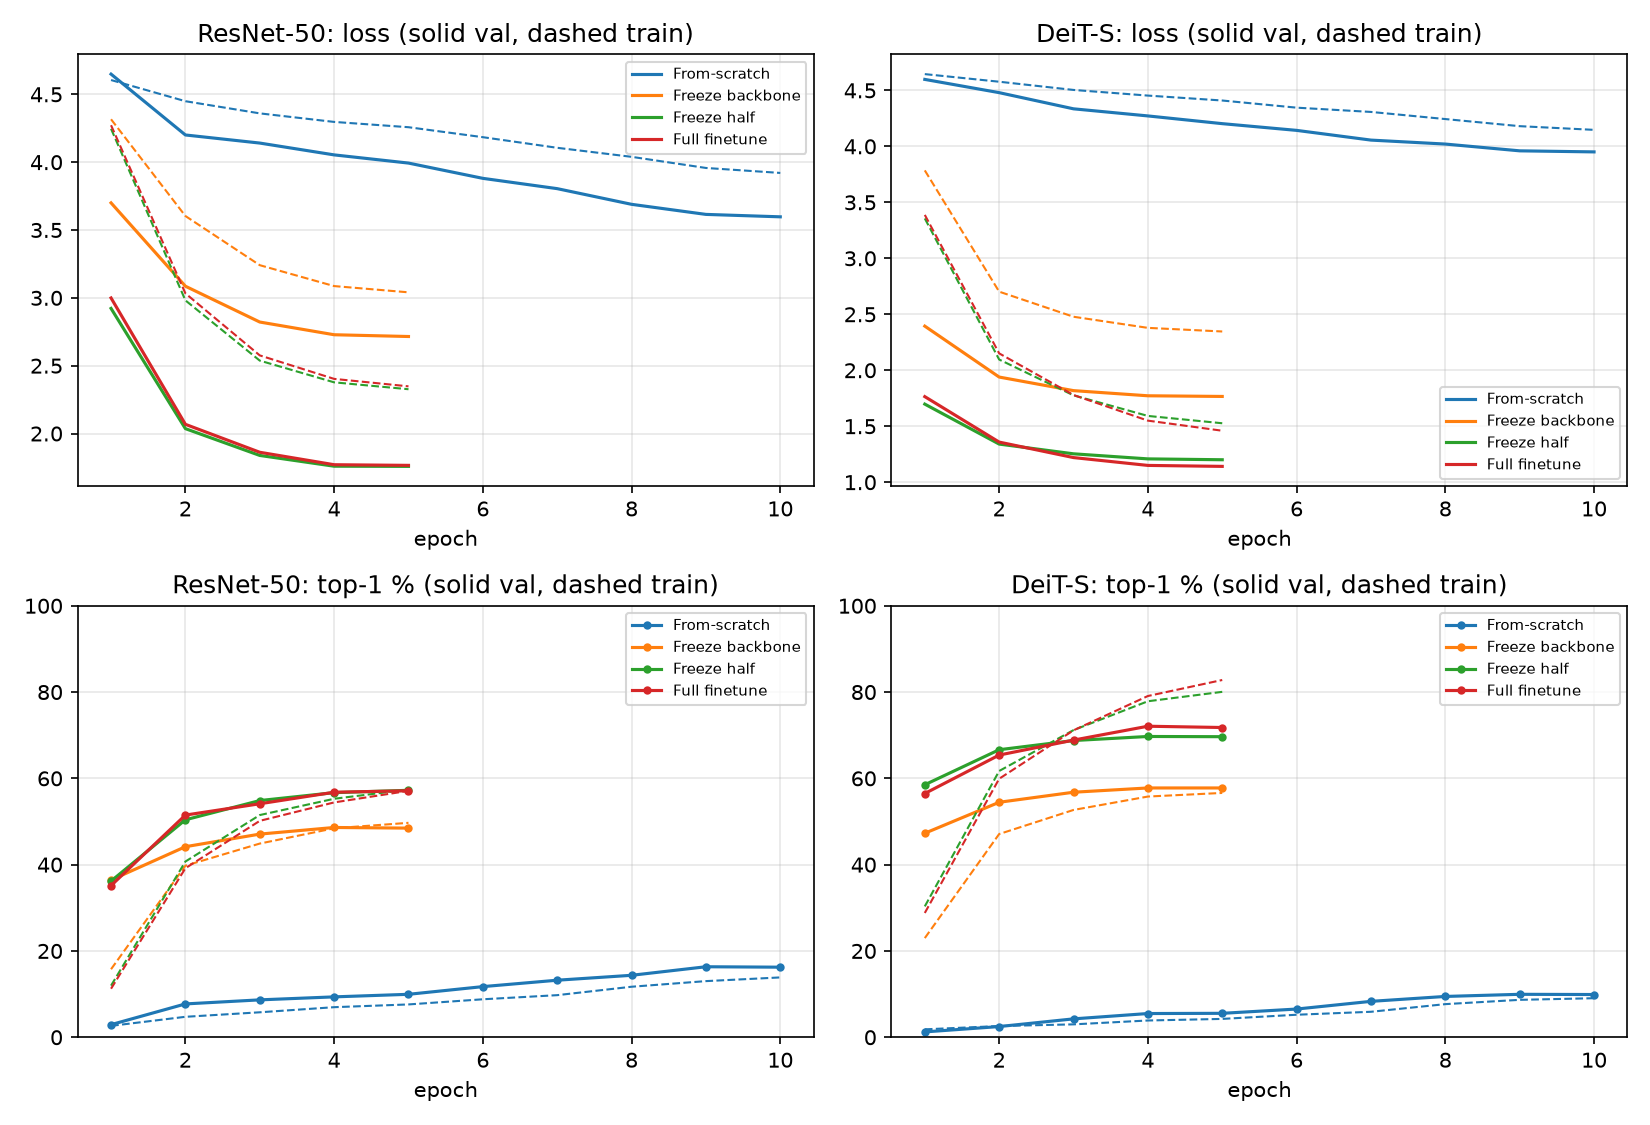
\includegraphics[width=\linewidth]{fig_curves.png}
  \caption{Loss (hàng trên) và top-1 (hàng dưới) theo epoch. Nét liền: validation; nét đứt: train. Accuracy train được đo trên ảnh đã augmentation, nên không so trực tiếp được với validation.}
  \label{fig:curves}
\end{figure}

\subsection{Accuracy và chi phí}

\begin{figure}[H]
  \centering
  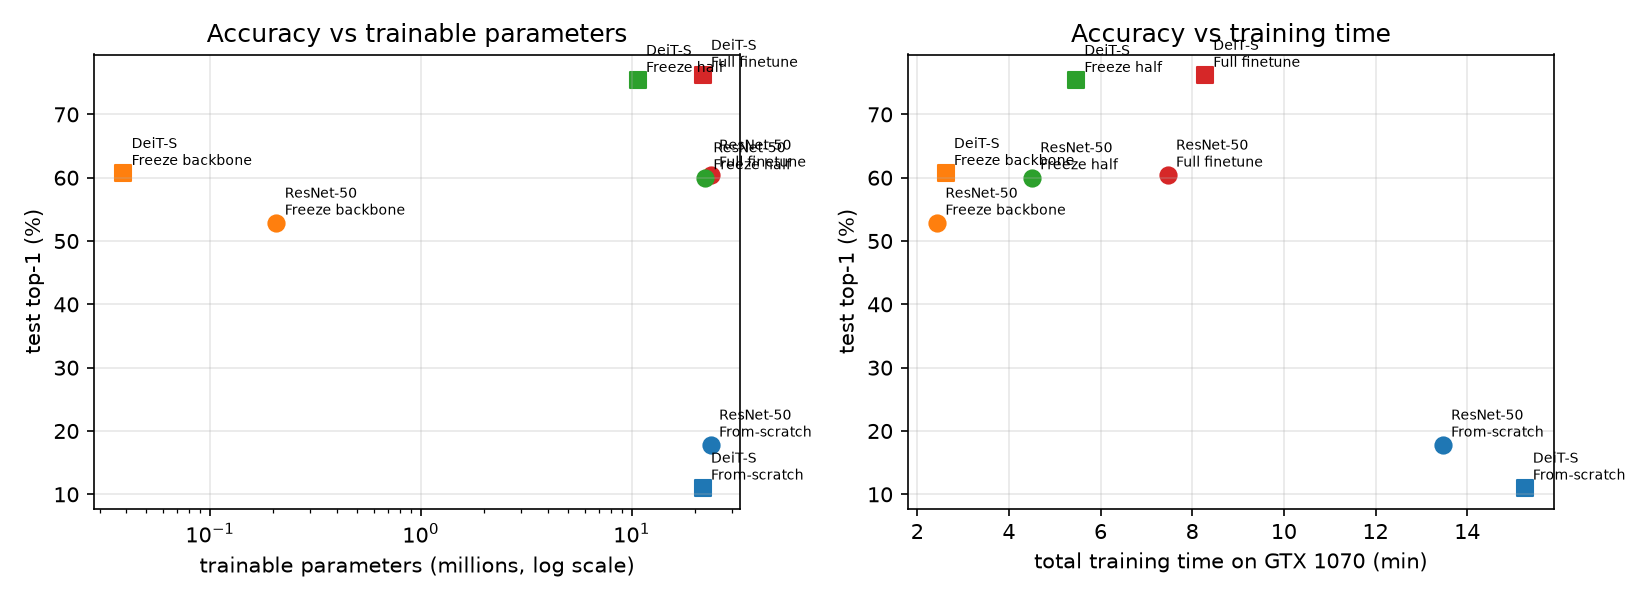
\includegraphics[width=\linewidth]{fig_acc_vs_cost.png}
  \caption{Top-1 trên test theo số tham số được train (trục log) và theo tổng thời gian train. Tròn: ResNet-50; vuông: DeiT-S.}
  \label{fig:acc-cost}
\end{figure}

\subsection{Phân tích lỗi}

Phân tích trên run tốt nhất của mỗi kiến trúc: ResNet-50 Full finetune (60,44\%) và DeiT-S Full finetune (76,20\%).

\begin{figure}[H]
  \centering
  \begin{subfigure}{0.49\linewidth}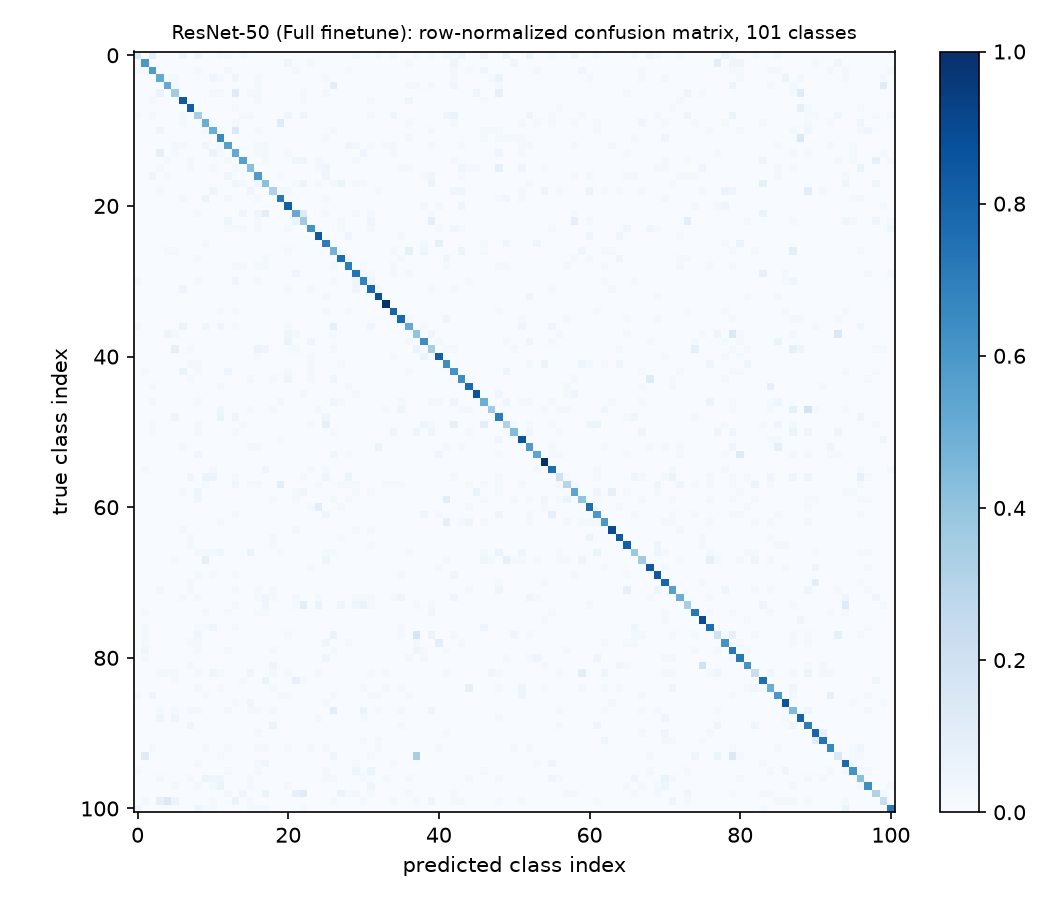
\includegraphics[width=\linewidth]{fig_confusion_resnet50.png}\end{subfigure}
  \begin{subfigure}{0.49\linewidth}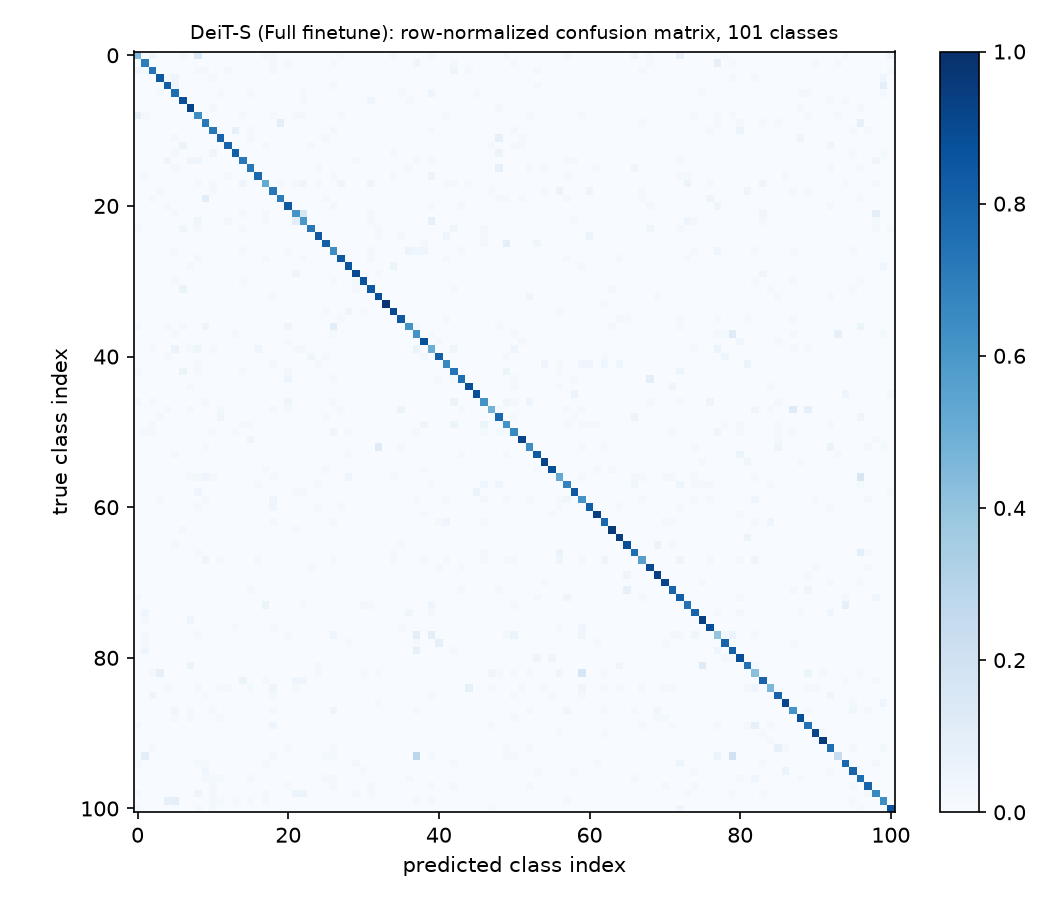
\includegraphics[width=\linewidth]{fig_confusion_deit_s.png}\end{subfigure}
  \caption{Confusion matrix chuẩn hóa theo hàng (101 lớp, theo thứ tự chữ cái). Đường chéo đậm hơn ở DeiT-S.}
  \label{fig:confusion}
\end{figure}

\begin{table}[H]
  \centering
  \caption{Các cặp lớp bị nhầm nhiều nhất trên test (thật $\rightarrow$ dự đoán, số ảnh trên 50).}
  \label{tab:confused}
  \small
  \begin{tabularx}{\linewidth}{lY}
    \toprule
    \textbf{Mô hình} & \textbf{Cặp nhầm nhiều nhất} \\
    \midrule
    ResNet-50 & steak $\rightarrow$ filet mignon (17), ramen $\rightarrow$ pho (10), gnocchi $\rightarrow$ shrimp and grits (9), pork chop $\rightarrow$ filet mignon (8), tuna tartare $\rightarrow$ beef tartare (7), steak $\rightarrow$ prime rib (7) \\
    \addlinespace
    DeiT-S & steak $\rightarrow$ filet mignon (14), steak $\rightarrow$ prime rib (10), ravioli $\rightarrow$ lasagna (8), huevos rancheros $\rightarrow$ tacos (8), chocolate cake $\rightarrow$ chocolate mousse (8), apple pie $\rightarrow$ bread pudding (7) \\
    \bottomrule
  \end{tabularx}
\end{table}

\begin{table}[H]
  \centering
  \caption{Năm lớp khó nhất và dễ nhất (accuracy trên 50 ảnh test mỗi lớp).}
  \label{tab:classes}
  \small
  \begin{tabularx}{\linewidth}{llY}
    \toprule
    \textbf{Mô hình} & & \textbf{Lớp} \\
    \midrule
    ResNet-50 & Khó nhất & apple pie (14\%), steak (14\%), pork chop (20\%), huevos rancheros (20\%), tuna tartare (22\%) \\
              & Dễ nhất  & hot and sour soup (100\%), edamame (100\%), macarons (90\%), pho (90\%), dumplings (88\%) \\
    \addlinespace
    DeiT-S    & Khó nhất & steak (24\%), pork chop (40\%), ravioli (42\%), apple pie (44\%), risotto (46\%) \\
              & Dễ nhất  & edamame (98\%), macarons (96\%), spaghetti carbonara (96\%), pho (94\%), oysters (94\%) \\
    \bottomrule
  \end{tabularx}
\end{table}

\begin{figure}[H]
  \centering
  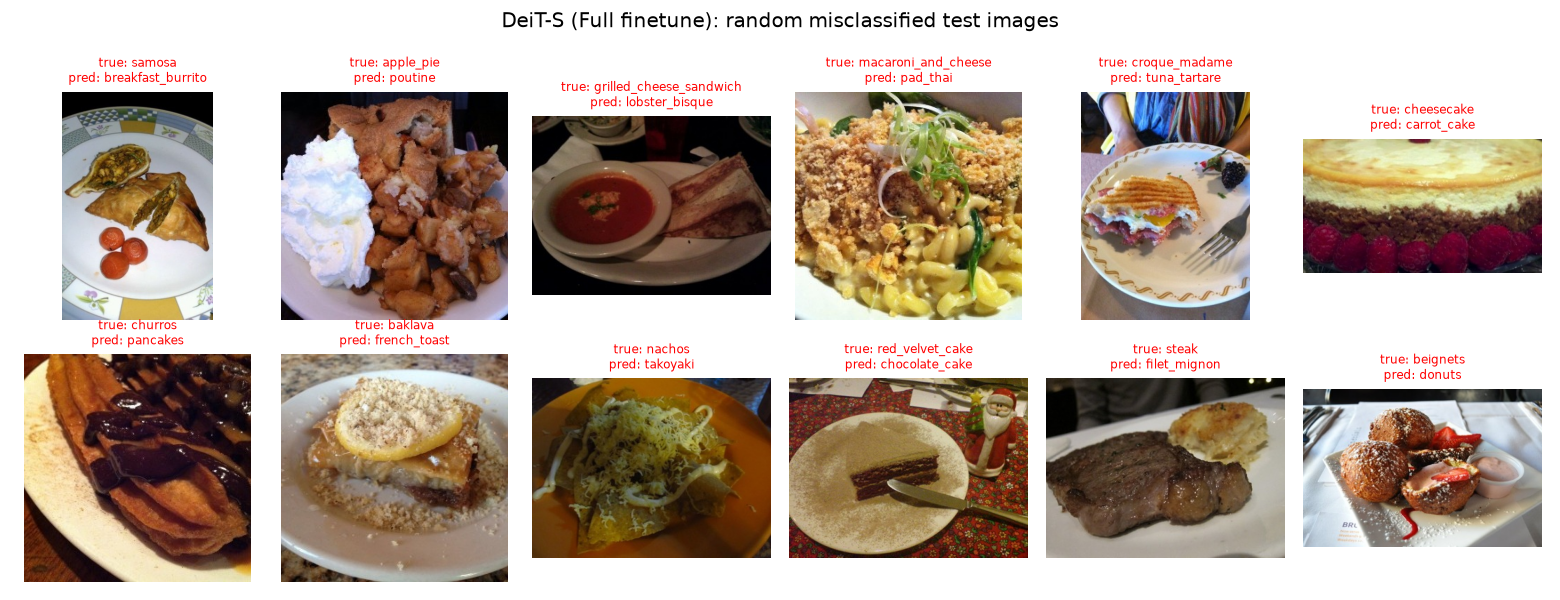
\includegraphics[width=\linewidth]{fig_errors_deit_s.png}
  \caption{12 ảnh test bị DeiT-S dự đoán sai, chọn ngẫu nhiên.}
  \label{fig:errors}
\end{figure}

\begin{itemize}
  \item \textbf{Lỗi tập trung ở các món giống nhau.} Cặp nhầm nhiều nhất của cả hai mô hình là steak $\rightarrow$ filet mignon; các cặp khác cũng là món cùng nguyên liệu hoặc cùng cách trình bày (ramen và pho, ravioli và lasagna, tuna tartare và beef tartare). Các lớp này chỉ khác nhau ở chi tiết nhỏ hoặc ở cách gọi tên, như Food-101 được thiết kế để thử phân loại chi tiết.
  \item \textbf{Hai mô hình khó và dễ ở cùng các lớp.} Steak, apple pie và pork chop nằm trong nhóm khó nhất của cả hai; edamame, pho, macarons và hot and sour soup nằm trong nhóm dễ nhất, vì có màu sắc và hình dạng đặc trưng. DeiT-S nâng các lớp khó nhiều nhất (apple pie và pork chop từ 14--20\% lên 36\%), nhưng steak vẫn dưới 20\% ở cả hai.
  \item \textbf{Một phần lỗi do chính dữ liệu.} Trong Hình~\ref{fig:errors}, một số ảnh sai có nhiều món trên cùng đĩa, chụp gần một phần món ăn hoặc thiếu sáng; một số nhãn khó xác định ngay cả với người xem. Mỗi lớp chỉ có 50 ảnh test, nên accuracy theo lớp dao động khoảng $\pm 7$ điểm và chỉ nên đọc như xu hướng.
\end{itemize}



% =====================================================================
\section{Thảo luận}

\subsection{CNN và ViT khi train from-scratch}
ResNet-50 đạt 17,80\% và DeiT-S đạt 11,01\%, nên ResNet-50 tốt hơn khi không có pretrain, và cách biệt 6,8 điểm lớn hơn nhiều so với sai số đo. ResNet-50 có sẵn inductive bias cục bộ và bất biến tịnh tiến, nên học được đặc trưng dùng được (cạnh, màu, kết cấu) ngay từ ít dữ liệu; DeiT-S phải tự học cả cách các patch liên hệ với nhau chỉ từ 10.100 ảnh.
Cả hai còn rất xa các run pretrained và validation vẫn đang tăng ở epoch cuối (ResNet-50: 16,2\%, DeiT-S: 9,9\%, epoch tốt nhất là 9 và 9), tức là 10 epoch trên 10.100 ảnh chưa đủ để hội tụ. Kết quả này chỉ nói về giai đoạn đầu của quá trình học, không phải mức trần của mỗi kiến trúc.

\subsection{Vai trò của pretrain}
Pretrain ImageNet là yếu tố lớn nhất trong toàn bộ thí nghiệm: full finetune hơn from-scratch 42,6 điểm với ResNet-50 và 65,2 điểm với DeiT-S, trong khi chỉ train 5 epoch thay vì 10. Mức tăng của DeiT-S lớn hơn ResNet-50 khoảng 22,6 điểm: không có pretrain thì DeiT-S kém ResNet-50, có pretrain thì vượt ở mọi chế độ. Điều này khớp với nhận định của ViT~\cite{dosovitskiy2021vit} và DeiT~\cite{touvron2021deit} rằng Transformer cần pretrain trên dữ liệu lớn nhiều hơn CNN. Ngay cả linear probe, chỉ train 206,949 (ResNet-50) và 38,885 (DeiT-S) tham số trong khoảng 2,5 phút, cũng vượt from-scratch hơn 35 điểm.

\subsection{Khi nào nên freeze}
\begin{itemize}
  \item \textbf{DeiT-S:} freeze backbone 60,69\%, freeze một nửa 75,39\%, full finetune 76,20\%. Mở khóa nửa sau tăng 14,7 điểm; mở thêm nửa đầu chỉ tăng 0,8 điểm, nằm trong sai số đo (khoảng $\pm 0{,}6$ điểm với 5.050 ảnh test). Freeze một nửa vì thế là điểm cân bằng tốt nhất: train 10,7M thay vì 21,7M tham số, mất 5,5 thay vì 8,3 phút và 1,3 thay vì 2,4 GB. Các block đầu của ViT học đặc trưng chung (cạnh, màu, kết cấu) dùng lại được cho món ăn; các block sau cần thích nghi với 101 lớp mới.
  \item \textbf{ResNet-50:} freeze backbone 52,85\%, freeze một nửa 60,02\%, full finetune 60,44\%. Freeze một nửa và full finetune ngang nhau. Phần bị khóa (\code{conv1} đến \code{layer2}) chỉ chứa khoảng 6\% tham số nhưng xử lý feature map độ phân giải cao, nên khóa nó giảm thời gian train từ 7,5 xuống 4,5 phút mà không mất accuracy.
  \item \textbf{Freeze toàn bộ backbone} rẻ nhất (khoảng 2,5 phút, DeiT-S chỉ cần 0,3 GB) và hợp khi cần một baseline nhanh hoặc rất ít dữ liệu, nhưng mất 7,6 điểm (ResNet-50) và 15,5 điểm (DeiT-S) so với full finetune: đặc trưng ImageNet không đủ để phân biệt các món ăn gần nhau nếu không được điều chỉnh.
\end{itemize}

\subsection{Vì sao DeiT-S vượt ResNet-50 khi có pretrain}
Ở cả ba chế độ pretrained, DeiT-S cao hơn ResNet-50 từ 7,8 đến 15,8 điểm, dù hai checkpoint có top-1 trên ImageNet gần bằng nhau (khoảng 80\%). Thí nghiệm này chưa đủ để kết luận nguyên nhân; các giả thuyết hợp lý là: (1) self-attention toàn cục hữu ích với ảnh món ăn, nơi lớp phụ thuộc vào bố cục và kết cấu của cả đĩa thay vì một vật thể cục bộ; (2) checkpoint \code{resnet50.a1\_in1k} được train với công thức rất mạnh và loss nhị phân~\cite{wightman2021rsb}, có thể chuyển giao sang tập mới kém hơn checkpoint ResNet-50 thông thường; (3) với ResNet-50, learning rate backbone $10^{-4}$ và 5 epoch có thể quá ít (validation vẫn tăng ở epoch cuối). Kiểm tra (2) và (3) cần thêm run với checkpoint torchvision và lịch train dài hơn.

\subsection{Đánh đổi accuracy và chi phí}
Tốc độ suy luận của hai mô hình gần bằng nhau (khoảng 410--490 ảnh/s trên GTX 1070), nên khác biệt chi phí nằm ở lúc train. DeiT-S dùng ít bộ nhớ GPU hơn ResNet-50 ở mọi chế độ (full finetune: 2,4 so với 5,3 GB), vì ResNet phải lưu các feature map lớn ở độ phân giải cao cho backward, còn DeiT-S chỉ lưu 197 token 384 chiều mỗi tầng; con số của ResNet còn gồm workspace của cuDNN. Trên Hình~\ref{fig:acc-cost}, DeiT-S freeze một nửa nằm gần góc tốt nhất: gần bằng accuracy cao nhất với chi phí thấp hơn full finetune.

\subsection{Hạn chế}
\begin{itemize}
  \item Quy mô nhỏ hơn protocol: 100 ảnh train mỗi lớp, 5 hoặc 10 epoch. Hai run from-scratch chưa hội tụ; khoảng cách giữa from-scratch và pretrained ở đây lớn hơn so với khi train đủ lâu.
  \item Một seed duy nhất; sai số chuẩn của top-1 trên test khoảng 0,6--0,7 điểm, nên các chênh lệch dưới khoảng 2 điểm (ResNet-50 freeze một nửa so với full finetune, DeiT-S freeze một nửa so với full finetune) không có ý nghĩa thống kê.
  \item Hyperparameter lấy theo protocol, không tinh chỉnh riêng cho từng mô hình.
\end{itemize}

% =====================================================================
\section{Kết luận}

Trên Food-101 với 100 ảnh train mỗi lớp: (1) pretrain ImageNet quan trọng hơn lựa chọn kiến trúc, đóng góp 43--65 điểm top-1; (2) khi có pretrain, DeiT-S vượt ResNet-50 ở mọi chế độ, tốt nhất 76,20\% so với 60,44\%; (3) không có pretrain thì ngược lại, ResNet-50 tốt hơn DeiT-S (17,80\% so với 11,01\%): ViT cần pretrain nhiều hơn CNN; (4) freeze một nửa backbone là lựa chọn hiệu quả nhất: accuracy ngang full finetune trong sai số đo, với thời gian train và bộ nhớ thấp hơn rõ rệt.

% =====================================================================
\section*{Tái lập kết quả}
\addcontentsline{toc}{section}{Tái lập kết quả}
Code: \url{https://github.com/hwnghoang/cs_deeplearning/tree/main/A1}. Từ thư mục \code{A1/}: \code{python scripts/prepare\_data.py} (split và resize), \code{python run\_all.py} (8 run, log và kết quả trong \code{results/}), \code{python -m src.analyze} (bảng và hình). Môi trường và các bước tải dữ liệu: \code{A1/README.md}.

\bibliographystyle{plainnat}
\bibliography{refs}

\end{document}
